% LaTeX Template für Abgaben an der Universität Stuttgart
% Autor: Sandro Speth
% Bei Fragen: Sandro.Speth@studi.informatik.uni-stuttgart.de
%-----------------------------------------------------------
% Hauptmodul des Templates: Hier können andere Dateien eingebunden werden
% oder Inhalte direkt rein geschrieben werden.
% Kompiliere dieses Modul um eine PDF zu erzeugen.
% Dokumentenart. Ersetze 12pt, falls die Schriftgröße anzupassen ist.
\documentclass[12pt]{scrartcl}
% LaTeX Template für Abgaben an der Universität Stuttgart
% Autor: Sandro Speth
% Bei Fragen: Sandro.Speth@studi.informatik.uni-stuttgart.de
%-----------------------------------------------------------
% Modul fuer verwendete Pakete.
% Neue Pakete einfach einfuegen mit dem \usepackage Befehl:
% \usepackage[options]{packagename}
\usepackage[utf8]{inputenc}
\usepackage[T1]{fontenc}
\usepackage[english]{babel}
\usepackage[backend=bibtex]{biblatex}
\usepackage{graphicx}
\usepackage[pdftex,hyperref,dvipsnames]{xcolor}
\usepackage{listings}
\usepackage[a4paper,lmargin={2cm},rmargin={2cm},tmargin={3.5cm},bmargin = {2.5cm},headheight = {4cm}]{geometry}
\usepackage{amsmath,amssymb,amstext,amsthm}
\usepackage[lined,algonl,boxed]{algorithm2e}
\usepackage{tikz}
\usepackage{hyperref}
\usepackage{url}
\usepackage[inline]{enumitem} % Ermöglicht ändern der enum Item Zahlen
\usepackage[headsepline]{scrpage2}
\usepackage{listings} 
\pagestyle{scrheadings} 
\usetikzlibrary{automata,positioning}
\hypersetup{hidelinks,
	colorlinks=true,
	allcolors=black,
	pdfstartview=Fit,
	breaklinks=true}
	
\colorlet{punct}{red!60!black}
\definecolor{background}{HTML}{EEEEEE}
\definecolor{delim}{RGB}{20,105,176}
\colorlet{numb}{magenta!60!black}

\lstdefinelanguage{json}{
    basicstyle=\normalfont\ttfamily,
    numbers=left,
    numberstyle=\scriptsize,
    stepnumber=1,
    numbersep=8pt,
    showstringspaces=false,
    breaklines=true,
    literate=
     *{0}{{{\color{numb}0}}}{1}
      {1}{{{\color{numb}1}}}{1}
      {2}{{{\color{numb}2}}}{1}
      {3}{{{\color{numb}3}}}{1}
      {4}{{{\color{numb}4}}}{1}
      {5}{{{\color{numb}5}}}{1}
      {6}{{{\color{numb}6}}}{1}
      {7}{{{\color{numb}7}}}{1}
      {8}{{{\color{numb}8}}}{1}
      {9}{{{\color{numb}9}}}{1}
      {:}{{{\color{punct}{:}}}}{1}
      {,}{{{\color{punct}{,}}}}{1}
      {\{}{{{\color{delim}{\{}}}}{1}
      {\}}{{{\color{delim}{\}}}}}{1}
      {[}{{{\color{delim}{[}}}}{1}
      {]}{{{\color{delim}{]}}}}{1},
}


% LaTeX Template für Abgaben an der Universität Stuttgart
% Autor: Sandro Speth
% Bei Fragen: Sandro.Speth@studi.informatik.uni-stuttgart.de
%-----------------------------------------------------------
% Modul beinhaltet Befehl fuer Aufgabennummerierung,
% sowie die Header Informationen.

% Überschreibt enumerate Befehl, sodass 1. Ebene Items mit
%\renewcommand{\theenumi}{(\alph{enumi})}
% (a), (b), etc. nummeriert werden.
%\renewcommand{\labelenumi}{\text{\theenumi}}

% Formatierung der Kopfzeile
% \ohead: Setzt rechten Teil der Kopfzeile mit
% Namen und Matrikelnummern aller Bearbeiter
\ohead{Sandro Speth\\
Markus Zilch\\
Dominik Wagner
}
% \chead{} kann mittleren Kopfzeilen Teil sezten
% \ihead: Setzt linken Teil der Kopfzeile mit
% Modulnamen, Semester und Übungsblattnummer
\ihead{Smart Cities and Internet of Things\\
Wintersemester 18/19\\
Specification}
\bibliography{bibliography.bib}
\title{Practical course
\\ Smart Energy Systems\\
	Report}
\date{Wintersemester 18/19}
\author{Sandro Speth\\
Markus Zilch\\
Dominik Wagner}

% Beginn des eigentlichen Dokuments
\begin{document}
\maketitle
\section{Introduction}

The traditional power grid is changing more and more over time.
Due to increasing sensititization for the use of renewable and reliable sources of energy instead of nuclear power sources, there is an increasing accomodation of renewable energy.
To fullfill our daily energy need only with such energy sources is quite difficult and needs lot of planning and simulation.
In this work we build a smart energy system to simulate a smart grid.

A smart grid is an energy efficient system with information and communication technology, automation and awareness of energy consumtion.
There are many different actors and technologies which are connected to each other and interoperate to optimate the grid.
%TODO Add "`Introduction to smart energy systems"' smart grid slides definitions

A smart energy systems creates the bridge between a power grid and a resilient and reliable smart grid.
Users can simulate reliable energy sources, as well as different kinds of energy consumers, e.g. homes or offices.
Simulation of distributed energy sources and automation of processes build an energy management system.
Through this microgrids we can possibly rely completly on renewable energy sources in the future.
This can be checked with our smart energy system.

The report is structured as follows.
In section \ref{sec:systemdesign} we present our system design.
First, we give some basic foundations which are relevant for our smart energy system, such as the difference between $kWh$ and $kW$.
Afterwards we present our functional requirements for the smart energy systems as user stories.
From these functional requirements we created our architecture which will be described in this section as well.



\section{System Design}\label{sec:systemdesign}

\subsection{Difference between $kW$ and $kWh$}\label{sec:diffEnergy}
W is a measuring scale for energy applied per time instance.
There are different possibilities to describe $W$ in common terms.
A pretty graphic one is the movement of mass.
$1W$ equals $1kg$ of mass moved by 1 meter in one second: $1 \frac{kg*m^2}{s^3}$.
Or in electrical terms: $1W$ equals 1 Ampere of electrical power with a voltage of 1 Volt.
Both of those formulas are equal to a much simpler Term for Watt: $1 W = 1 J/s$.
In simple terms, 1 Watt is the same as one Joule of energy applied over 1 second.
For completeness, $1kW = 1000 W$ \cite{Nelson,Borvon,SIStandard}.

$Wh$ are the common term for measuring energy consumption and production.
$1Wh$ is $1W$ applied continuously over 1 hour.
$1Wh = 1 W * 1h = 1 J/s * 3600s = 3600J$.
For a scientific context the $Wh$ therefore is simply not used, instead the common SI standard $J$ is used.
In comparison, $Wh$ is the total amount of energy used. $W$ is how much energy is used in a specified timeslot (mostly 1 second) \cite{EURichtlinie,Bundesgesetz}.


\subsection{Difference between consumption and demand}\label{sec:diffconsumptiondemand}
Electricity consumption and electricity demand are two different properties and measured with different measurement units.
The following section contains a description of both and an example at the end.

\subsubsection{Demand}

The demand is the rate of consumption of electricity or mathematical speaking the demand is the derivation of the consumption [1]. %\cite{https://www.stonybrook.edu/commcms/energy/facts/demand}. 
Most of the time the demand is measured in Watt. If you turn on a 100W light bulb, it will demand 100W while it is turned on. At the same time the grid must provide electricity at a rate of 100W. In most cases it is possible to calculate the demand with the following formula [2]. %http://www.iris.uni-stuttgart.de/lehre/eggenberger/eti/index.html
\begin{equation*}
	Demand = Voltage * Current
\end{equation*}
Some customers also have to pay for the demand or peak demand they have because if you have a higher (peak) demand the grid has to support this [1,3].  %https://www.enertiv.com/resources/what-is-peak-demand,https://www.stonybrook.edu/commcms/energy/facts/demand


\subsubsection{Consumption}

It is easier to understand electricity consumption because we are more used to this concept [1]. Many people deal with electricity consumption while paying their electricity bill because most German electricity meter measure only the consumption. %\cite{https://www.stonybrook.edu/commcms/energy/facts/demand}.
The consumption is the amount of electricity used per time unit [1,3]. Most of the time the consumption is measured in kilowatt per hour.
The formula to calculate the consumption is the following [1]. %https://www.stonybrook.edu/commcms/energy/facts/demand.

\begin{equation*}
	Consumption = Demand * Time
\end{equation*}
For example, 5 W LED bulbs turned on for 1h have the consumption of 5 Wh.
\subsubsection{Difference}

The demand is the rate of which we use energy and the consumption is the total energy used for a given time frame [1]. If someone turns on 1 heating unit with a demand of 1kW for 2 hours than the demand during this hours is 1kW, but the consumption is 2kWh. The consumption is the same if two heating units are used for half an hour, but the demand is doubled (2kW). To put it in simple terms the demand is comparable with the speed of a car and the consumption is the distance you drive. The faster you drive the more distance is accumulated over time.\\\\ %https://www.stonybrook.edu/commcms/energy/facts/demand


[1] Consumption Vs. Demand - Stony Brook University https://www.stonybrook.edu/commcms/energy/facts/demand

[2] Leistung des elektrischen Stroms - Prof. Dr. Otto Eggenberger - Universität Stuttgart 
http://www.iris.uni-stuttgart.de/lehre/eggenberger/eti/index.html

[3] What is Peak Demand? - enertiv https://www.enertiv.com/resources/what-is-peak-demand





\subsection{Userstories}\label{sec:userstories}
\begin{enumerate}
\item As a user, I need to create one or more wind turbines in the simulation so that I can calculate the potential energy output.

\item As a user, I need to create one or more photovoltaic panels in the simulation so that I can calculate the potential energy output.

\item As a user, I need to create one or more batteries in the simulation so to save unused energy of in my simulation.

\item As a user, I need to get the charge state of my batteries to know the impact of the energy storage on the grid.

\item As a user, I need to create one or more homes on the demand side in the simulation so that I can simulate some energy consumer.

\item As a user, I need to create one or more commercial buildings on the demand side in the simulation so to simulate some high energy consumer.

\item As a user, I need to get dynamic energy prices calculated from the simulation to determine if I want to sell my produced energy or store it for later use.

\item As a user, I need to use weather data in the simulation to simulate the smart energy system more precise and realistic.

\item As a user, I need to use already saved weather data in the simulation to not be dependent on the availability of the weather service.

\item As a user, I need to generate a forecast for energy generation and demand using the simulation in order to make informed decisions.

\item As a developer, I want to add more supplier modules than wind tubines and photovoltaic pannels to the simulation to improve the smart energy system in the future with further technology due to adding more kind of supplier. 

\item As a developer, I want to add more consumer modules to the simulation to be able to add more kinds of consumers to the simulation. 

\item As a user, I want to be able to create a smart energy system which is independent to an power grid to simulate a reliable smart grid.

\item As a user, I want to get a visual notification if the supply of energy is smaller than the demand of energy to know when more energy supplier are needed.

\item As a demand module, I need to get energy from the (charged) batteries if the provided supply to small for my demand so that I still have enough money. 

\item As a user, I want to model a rechargeable battery so I can store the energy for later usage, if the supply is greater than the demand.

\item As a user, I need the battery to be able to discharge energy if the supply is lower than the demand in order to make my stored energy usable and keep the demand satisfied.

\item As a user, I need the smart grid to be able to manage peaks in the demand in order to smooth the impact on the grid and reduce the likelyhood of power outages.

\item As a user, I need that the demand side consumers feature different load scenarios like home users and commercial users (constant load, occasionally peak loads) in order to make the simulation accurate for real life applications.

\item As a user, I want be able to use the system with my webbrowser so that I can use different platforms to view it and have easy access to the simulated data.

\item As a user, I want to be able to see the energy supply of each individual supply component in order to be able to assess the efficiency of the supplier.

\item As a user, I want to be able to see the energy demand of individual components for efficiency assessment and informed decision making. 

\item As a user, I want to see a summary of energy supply and demand for all components in order to easily assess the current situation.

\item As a user, I want to adjust the demand by postponing the use of devices during peak hours in order to prevent a complete outage of the grid or to react to one-time-only scenarios.

\item As a user, I want the simulation to adapt the demand based on the price per kWh in order to minimize costs of my energy demands and maximize profits of my energy supply.

\end{enumerate}



\subsection{Architecture}
The weather component is the component responsible for looking up weather data for registered supply and demand components.
The component reads registration data from the database and looks up weather data for each recorded entry.
The collected data is written back into the database in order to be usable for the rest of the system.\\
\\
In order for the whole system to be reliable and responsive we devided the weather component from the rest of the system.
The weather component speaks only to the weather database where it get the locations for which it should collect weather data.
The collected data gets written into the database and stored.
Even in the case of a failure of the weather component the already collected data is still accessible and therefore the system can still access it, making the system independent of the weather component.
In the case of a new registration of a component during a weather component failure, the database may return default values for the new component in a way the running system is not being halted by missing data.
These measures should make the system reliable and and responsive in that context.\\
\\
The three-layered architecture was already planned for in the first conceptions of the project, therefore no extra steps had to be taken.
We divided the project in subcomponents and put them in the respective part of the architecture.\\
The first layer is the data layer which only consists of data-providing hardware and databases. Since the current project does not include data-providing hardware (as far as the current conception goes) only databases are left in this layer.\\
The second layer consists of the functional components of the project.
All suppliers, storages, consumers and utility components are part of this layer, since they mostly take data from the databases and compute their respective power in- and output based on those values and give them to the simulation component.
The simulation component is part of this layer, and takes the data the other component in order to model the different interactions of the smart grid.
The workflow is controlled by the controller component and connects all components together.
The last component in this layer is the REST component which makes the computed data from the simulation component available to the frontend layer.\\
The frontend layer is the third and last layer in our project.
It handles the interaction with the user and makes it possible for the user to add and remove components to the smart grid simulation as he sees fit.

\section{Implementation}\label{sec:Implementation}
\subsection{Gather weather design}
\subsubsection{Weather service}\label{sec:weatherservice}
For our smart energy system, we need a weather service which can provide all needed data on an hourly basis.
There is one weather service which fulfills our needs more than appropriate.
The weather service \url{weatherbit.io} has different kinds of endpoints on its API.
In our case we use two of them, the current weather data API and the 48 hours weather forecast API.

Before we take a look at the endpoints provided to the user and their responses, we want to present the data collectable on weatherbit.io.
An example response of the current weather API is shown in listing \ref{lst:weatherdata}.
The property  \texttt{data} of the JSON object contains an array of weather data points.
For current weather API there is only one object in the array.
But for the forecast there are up to 48 objects, one for every hour of the forecast.
\begin{lstlisting}[caption={Example response of weatherbit.io for $lat=31.23$ and $lon=121.47$}, label={lst:weatherdata}, frame=single, language=json]
 {
    "data": [
        {
            "wind_cdir": "SSE",
            "rh": 100,
            "pod": "n",
            "lon": 121.47,
            "pres": 1012.2,
            "timezone": "Asia/Shanghai",
            "ob_time": "2018-11-07 20:35",
            "country_code": "CN",
            "clouds": 0,
            "vis": 10,
            "solar_rad": 0,
            "state_code": "23",
            "wind_spd": 0.89,
            "lat": 31.23,
            "wind_cdir_full": "south-southeast",
            "slp": 1013.2,
            "datetime": "2018-11-07:20",
            "ts": 1541622900,
            "station": "E7205",
            "h_angle": -90,
            "dewpt": 13.9,
            "uv": 0,
            "dni": 0,
            "wind_dir": 156,
            "elev_angle": -29.2797,
            "ghi": 0,
            "dhi": 0,
            "precip": null,
            "city_name": "Shanghai",
            "weather": {
                "icon": "c01n",
                "code": "800",
                "description": "Clear sky"
            },
            "sunset": "09:00",
            "temp": 13.9,
            "sunrise": "22:14",
            "app_temp": 13.9
        }
    ],
    "count": 1
}
\end{lstlisting}
From all those data we chose only to store \texttt{lat} for latitute, \texttt{lon} for longitute, \texttt{pres} for air pressure, \texttt{rh} for relative humidity, \texttt{ghi} for global horizontal solar irradiance, \texttt{wind\_spd} for wind speed, \texttt{temp} for the temperature, and the timestamp in UTC format.

The API for the current weather data returns current weather data of over 45.000 stations.
Every API request will return the nearest, and most recent observation.
There are several endpoints available in the API.
For example, a user can get current weather observation by lat/lon as we do or by city name.
All endpoints differ only on their required query parameters.
They define whether to get the observation by lat/lon, city name or any other possible way.
The basepath for all endpoints is \texttt{https://api.weatherbit.io/v2.0/current} and the supported method is \texttt{GET}.
To get the data in the metric format you have to add an additional query parameter \texttt{unit=m}.
Every request must provide an API key in query parameters.\cite{weatherbit}
This API key can be requested by creating an account on weatherbit.io.
After creating an account a user has to choose a pricing plan.
For our system the free plan is totally sufficient.

The API for the weather forecast data returns the weather forecast for up to 48 hours on an hourly basis.
Nevertheless, we only request it for 24 hours.
While the basepath is now \texttt{https://api.weatherbit.io/v2.0/forecast/hourly}, the provided query parameter are the same with an additional query parameter \texttt{hours} which must get a value between 0 and 48 to specify the size of the forecast.

\subsubsection{Our WeatherCollector service}\label{sec:weathercollector}
To gather weather data for different locations and store it into a database we build a service, which is under MIT licence available on GitHub\footnote{\url{https://github.com/smart-energy-system/WeatherCollector}}.
The service runs a NodeJS express server with two endpoints to create or delete \texttt{WeatherCollector} objects. 
A \texttt{WeatherCollector} object gathers every hour current weather data for a given location as well as 24 hours weather forecast on an hourly basis and stores the data in a database. 
While gathering new forecast data, the old deprecated data is getting replaced, so there is always the latest 24 hour forecast data. Multiple WeatherCollector objects are possible to collect weather data for different locations at the same time.

There are several dependencies you have to install before running the server. 
Since the code runs on NodeJS version 8 or higher with a current npm, you need to have this installed first.
First, run \texttt{npm install} to install needed dependency packages. 
You can look up the installed libraries and their versions in \texttt{package.json} file. 
After installing the packages, you need to create the database. 
Therefore, run \texttt{node DBCreator.js} to create the database file and required SQL tables. 
Now you are nearly ready to run the server.

You can test the functionality without running the complete server.
You just need to run \texttt{WeatherCollectorTest.js} to play around with some locations. 
On the first run of the module you need to provide it with your weatherbit.io API key, latitute and longitute of the location: \texttt{node WeatherCollectorTest.js "<API Key>" <lat> <lon> "<mode>"}. 
Keep in mind that you already need the API key requested from weatherbit.io.
There are 5 modes available to test:
\begin{itemize}
	\item \texttt{collect}: Collects a current weather data of the given location and stores it into the database
	\item \texttt{get}: Gets the latest stored current weather data of the given location
	\item \texttt{collect forecast}: Collects a 24 hour weather forecast on hourly basis for a given location and stores it into the database
	\item \texttt{get forecast}: Gets the latest version of the forecast weather data of the given location
	\item \texttt{start}: Starts a WeatherCollector object on hourly picking new weather data (current and forecast) and stores the data into the database.
\end{itemize}

If you did run the complete run command once, a test config file was created. 
So unless you want to change your API key or the location you can shorten the run command a bit, using only \texttt{node WeatherCollectorTest.js "<mode>"}.

You can simply run the server with \texttt{npm start <API key>}. 
This will create a config file with your API key, so later you can start the server just running \texttt{npm start} command.

Since the service is a REST service, there are two HTTP REST endpoints available on the server, one for creating WeatherCollector objects and one for deleting them.
To create a new WeatherCollector object, you can send an \texttt{POST} request against \texttt{<basepath>/weathercollectors} providing the body shown in listing \ref{lst:postbody} as content-type \texttt{application/json}. 
\begin{lstlisting}[caption={Body of \texttt{POST} request endpoint}, label={lst:postbody}, frame=single, language=json]
{ 
	"lat":<lat>, 
	"lon": <lon> 
}
\end{lstlisting} 
If \texttt{lat} and \texttt{lon} are correct and the object is created successfully you will get status 201 and a JSON object as shown in listing \ref{lst:postresponse} in return.
\begin{lstlisting}[caption={Body of the response of the \texttt{POST} request}, label={lst:postresponse}, frame=single, language=json]
{ 
	"lat": <lat>, 
	"lon":<lon>, 
	"id":<id> 
}
\end{lstlisting}
The \texttt{id} is the ID of the object created. 
You will need it to delete the object later, so better save it anywhere. 
After creating the object, the object is requesting the weather data (current and forecast) every hour. 
If one of the request body properties is not defined you will get a status 400 in return.

To delete a WeatherCollector object of given ID, you can send an \texttt{DELETE} request against \texttt{<basepath>/weathercollectors} providing the in body the data shown in listing \ref{lst:deletebody} as content-type \texttt{application/json}.
\begin{lstlisting}[caption={Body of \texttt{DELETE} request endpoint}, label={lst:deletebody}, frame=single, language=json]
{ 
	"id":<id> 
}
\end{lstlisting}
If \texttt{id} is set and there is a WeatherCollector object with such an ID, it will be deleted and therefore stops gathering data. 
The return will be status 200. 
If id is not set or there is no WeatherCollector object with such an ID, the return will be status 400.




\subsection{Windturbine}
\subsubsection{Swept area function}
The swept area of a windturbine is dependent on the radius of the rotary blades. Combined with the constant Pi the area swept can be computed by the equation: $A = r^{2}* \Pi $\\
Source: $Beckmann, Petr (1976), A History of Pi, St. Martin's Griffin, ISBN 978-0-312-38185-1$
\subsubsection{Vapor pressure}
To compute the actual vapor pressure in the air the relative humidity has to be given. The relative humidity is computable with the equation $H = P_{av} / P_s$ with $P_{av}$ being the actual vapor pressure and $P_s$ being the saturated vapor pressure at a given temperature. This equation can be restructured to get the actual vapor pressure: $P_{av}  = H * P_s$. The relative humidity is a parameter for the function, which is filled with data form the before mentioned weather data collection.\\
\\
To be able to now compute the actual vapor pressure at a given temperature we still need the saturated vapor pressure. For this we can use the Herman Wobus equation (E being the vapor pressure):\\
$E = e/p^{8}$ with\\
e = 6.1078 and\\
$p = c_0 + T * (c_1 + T * (c_2 + T * (c_3 + T * (c_4 + T *(c_5 + T * (c_6 + T * (c_7 + T * c_8 + T * c_9)))))))$\\
with $c_0$ to $c_9$ being constants and T being the temperature in degrees Celsius.\\
Source: $http://www.emd.dk/files/windpro/WindPRO_AirDensity.pdf$
\subsubsection{Density of moist air}
In order to compute the density of moist air, we have to have a look at how it is compounded. Moist air density is a mixture of dry air and water vapor. The physical equation for this is: $D_m = (P_d/(R_d * T_k))+(P_v/(R_v*T_k))$\\
$D_m$ is the density of moist air, $P_d$ is the pressure of dry air at the specified temperature, $R_d$ is the gas constant for dry air, $P_v$ is the pressure of water vapor at the specified temperature, $R_v$ is the gas constant for water vapor and $T_k$ is the given temperature in degrees Kelvin. With the previously implemented methods this equation system is able to compute the air density with only the temperature and relative humidity given.\\
Source: $Shelquist, R (2009) Equations - Air Density and Density Altitude$\\
Source: $http://www.emd.dk/files/windpro/WindPRO_AirDensity.pdf$
\subsubsection{Wind turbine model}
The wind turbine model contains some variables which can be set by the user. The function for computing the generated energy is derived from the power coefficient of the turbine (basically the efficiency), the size of the turbine (shows in area swept), the density of the air in the area and of course the weather conditions which apply at the moment given.
The general equation for this setup is: $P_{avail} = (1/2) * p * A * v^{3} * C$
where p is the air pressure, A the area swept, v the windspeed and C the power coefficient.\\
Source: $https://www.raeng.org.uk/publications/other/23-wind-turbine$
\subsection{Photovoltaic}
\subsubsection{Temperature loss}
The function for the temperature loss is giving a linear function for the percentage loss of energy depending on the degrees over 25 degree Celsius. We made the assumption the efficiency does not go over 100 \% even for temperatures below 25 degree Celsius.The resulting equation is as follows: $L_t = max((T-25)*0.005 , 0)$ with the result being the percentage of energy lost due to temperature as a point number.
\subsubsection{Performance Ratio}
The performance ration is computed with the equation $1.0 - (\text{total percentage of losses})$.
With the previous computed losses for temperature and the constant loss $L_0$ of 0.14 we get the equation $R = 1.0 - (L_0 + L_t) = 1.0 - (0.14 + L_t)$
\subsubsection{Solar irradiance}
The computation of the SolarRadiationIncident and therefore the effective Solarradiation on the surface of the solarpanel can be computed with the equation $(SP_{horizontal} * sin(\alpha + \delta))/sin(\alpha)$.
$\alpha$ is the effective tilt of solarradiation on a specified latitude and set as 90 - Latitude of the object + $\delta$.
$\delta$ is the tilt of the solarradiation in regard of the day of the year d and can be computed with the following equation: $23.45 * sin((360/365) * (284 + d))$
Source: https://pveducation.org/pvcdrom/properties-of-sunlight/solar-radiation-on-a-tilted-surface
\subsubsection{Photovoltaic Model}
The formula for computing the generated energy as given in the slides is: $E = A * r * PR * S$\\
A is the area of the solarpanel and is given by the user in $m^{2}$.
Same goes for the solar panel yield r which is given by the user as well.
The performance ratio PR  is computed in on of the previous steps and is  a percentage.
S is the solar radiation incident and is computed in regards of solar radiation and other factors taken from the database.
The measurement unit for S is $W/m^{2]$.
The resulting unit for produced energy is therefore W.
\subsubsection{Battery Model}
The first function for returning the current state of the battery is a simple return of the currently stored energy.
The formula for charging and discharging is more complex and takes several parameters.
The parameters are charging and discharging rate as well as charging efficiency.
The function returns the actual change of energy stored in the battery.
The returned value is positive if the battery is charged and negative if the battery is discharged.
\subsubsection{Demand Profile}


\section{Demand Response and coordination}\label{sec:DemandResponse}
\subsection{Balance within the microgrid}
To guarantee the balance in the microgrid as defined in the slides we have to formulate a mathematical equation to use as a constraint.
We came up with the following equation:\\
\begin{align} \label{eq1:balance}
\begin{split}
\forall t \in T: \sum\limits_{s \in S}{P_{s}(t)} + \sum\limits_{b \in B}{P_{b}(t)} + P_{g}(t) = \sum_{h \in H}({P_{h}(t)} + PposShift_h(t) - PnegShift_h(t))
\\ + \sum_{c \in C}({P_{c}(t)} + PposShift_c(t) - PnegShift_c(t)) - \sum\limits_{b \in B}{Pd_{b}(t)}
\end{split}
\end{align}
As one can see, for all time steps $t$ in the set of all time steps $T$ the equation has to hold true. 
This is the constraint for the whole microgrid. 
The left side of the equation represents the power supplied by the supplier ($P_{s}(t)$), the batteries ($P_{b}(t)$) and the import or export from the main grid ($P_{g}(t)$), the right side represents the consumers, which contains of homes ($P_{h}(t)$) and commercial buildings ($P_{c}(t)$), the batteries ($Pd_{b}(t)$) while charging. 
On the right side, there are also the demand shift values for homes and commercial buildings.

If the balance between the consumers and the suppliers is disturbed, severe consequences can happen. 
Any imbalance results in a change in the frequency. 
This change may forces more suppliers to stop production because most suppliers can only operate in a narrow frequency range. 
As a result of this the imbalance ingresses even more. 
If the change in the frequency exceeds a certain threshold suppliers and consumers still connected to the grid could be damaged. 

The supply side of the equation itself is compartmentalized into different factors which are explained in the following.

\textbf{Wind turbines and solar panels:} On the supply side we have the sum the power in time step $t$ of all suppliers of the system (($P_{s}(t)$)), regardless of wind turbines or solar panels.
We get those values from our model given data for the time step and weather conditions. 
Our software calculates demand forecast and supply forecast based on models of the supplier and consumers. 
Additionally, the location of the installations are provided by the user and a weather forecast is provided by a weather service. 
For example, for the wind turbines, the Herman Wobus equation is used to calculate the saturated vapor pressure \cite{NOAA}. 
This equation is based on empirical data and helps us to incorporate the weather forecast in the wind supply forecast. 
Because all these calculations happen before the optimization step, the solver does not need to know anything about the specifics of the supplier or consumer. 
This supports reuse-ability of the solver and the models for it. 
The forecast data is provided as an array of data which contains a value for each time step. 
The values represent the supply or demand and are measured in $Watts$.  %TODO Auf welche Einheit haben wir uns jetzt entschieden?

\textbf{Battery supply:} The second part is the power provided by the sum of all batteries at a given time step $t$. % TODO wiederholt sich das nicht von oben?

\textbf{Import and export to the main grid:} The connection to the main grid is resolved in the third part of the supply side of the equation.
If we have more demand than supply, the solver will either use the energy stored in the battery or import energy from the main grid.
While the import of energy from the battery is already satisfied with the battery supply we can here import energy from the main grid which generates us some costs.

For the demand side, we chose a similar approach.

\textbf{Demand from homes and commercial buildings:} The first one is the sum over all homes of a a given time step $t$ with related demand shift of every single home to calculate the total demand of all homes.
The second one is the sum over all commecial buildings of a given time step $t$ with related demand shift of every single commecial building to calculate the total demand off all commecial buildings.
Comparable to the supply forecast, the demand forecast is generated before the optimization step. 
It is based on the demand profiles described in \cref{subsec:Demand}. 
The demand of the homes is provided as an array of constants to the solver and measured in $Watts$. 
Because the supply and the demand are provided as constants to the optimization component, we did not formulate any constraints for the supplier or the consumers.
For the demand shift parts of the demand entities we have a positive shift and a negativ shift.
The negative demand shift tells us how much demand is shifted away on this time step.
The positive demand shift tells us the opposite, how much demand is shifted to this time step.
So the negative demand shift will decrease the demand while the positive demand shift will increase the demand.
If the negative demand shift of a home or commecial building is greater than 0, the positive demand shift has to stay 0 and vice versa.

\textbf{Demand of batteries:}
The third part calculates the demand of all batteries at a given time step $t$.
If we have more supply than demand, the solver can either export the unnecessarily produced energy to the main grid or store it in a battery for later use.
The storage of energy in the battery has a small loss of energy.

\subsubsection{Additional Constraints}
There are additional constrains which have to hold true in our simulation. 
For example it is not possible to charge and discharge batteries at the same time.
TODO

\subsection{Objective of the optimization problem}
To maximize the profit in a specified interval of timesteps $t \in T$ between the time steps $a \in T$ and $b \in T$ we propose the following function:\\
\begin{equation} \label{eq:opt}
\max_{p \in P}{(\sum_{t=a}^{b}{((E(t)*price(t))-(I(t)*cost(t)))})}
\end{equation}
Where P is th set of all possible decision configurations. $E(t)$ and $I(t)$ are depending on the decisions made and on the equation for the balance in the microgrid of the exercises before. All configurations from P have to satisfy all the constraints. The formula consists of two main parts. The minuend in the sum calculates the profit for exporting energy to the main grid for these time step. For this calculation, the total energy export $E(t)$ for this time step is multiplied by the price for the energy. The subtrahend in the sum expresses the cost for importing energy from the main grid. It consists of the total imported energy $I(t)$ multiplied by the cost for importing energy at this time step. There are different possibilities to improve the total profit. For example, one could sell energy at a high price. Another possibility is to store energy if the price for selling is low. For our simulation we use time steps with the width of one hour, so the values for power and energy are the same, but $E(t)$ and $I(t)$ are measured in Wh while the unit of all values of the previous equation is Watt.

\subsection{Nomenclature Table}
	\begin{longtable}{|c|p{.50\textwidth}|c|c|}
		\toprule
		\textbf{Symbol} & \textbf{Description} & \textbf{Unit} & \textbf{Equation} \\ \midrule
		T & The set of all time steps. The step width is 1h and usually 24 steps are used. & Hour & \Cref{eq1:balance,eq:opt} \\ \midrule
		t & A single step from the set T. & Hour & \Cref{eq1:balance,eq:opt} \\ \midrule
		S & The set of all suppliers (Different wind turbines, solar panels...). & Watt & \Cref{eq1:balance} \\ \midrule
		s & A single supplier from the set S. & & \Cref{eq1:balance} \\ \midrule
		$P_{s}(t)$ & The energy supply from a single supplier for the specific time step t. & Watt & \Cref{eq1:balance} \\ \midrule
		B & The set of all batteries. & & \Cref{eq1:balance} \\ \midrule
		b & A single battery. & & \Cref{eq1:balance} \\ \midrule
		$P_{s}(t)$ & The energy supply from a single battery for the specific time step t. & Watt & \Cref{eq1:balance} \\ \midrule
		$P_{g}(t)$ & The energy supply from the main grid for the specific time step t. & Watt & \Cref{eq1:balance} \\ \midrule
		D & The set of all consumers (Homes, commercial buildings) & & \Cref{eq1:balance} \\ \midrule
		d & A single consumer from the set D & & \Cref{eq1:balance} \\ \midrule
		$P_{d}(t)$ & The energy demand for a single consumer at a specific time step t. & Watt & \Cref{eq1:balance} \\ \midrule
		$P_{b}(t)$ & The energy demand for a single battery at a specific time step t. & Watt & \Cref{eq1:balance} \\ \midrule
		$Pd_{g}(t)$ & The energy exported by the microgrid to the main grid at a specific time step t. & Watt & \Cref{eq1:balance} \\
		P & The set of all possible configurations &  & \Cref{eq:opt} \\ \midrule
		p & A single configuration &  & \Cref{eq:opt} \\ \midrule
		a & A single step form the set T. It marks the first time step of the optimization & Hour & \Cref{eq:opt} \\ \midrule
		b & A single step form the set T. It marks the last time step of the optimization & Hour & \Cref{eq:opt} \\ \midrule
		E(t) & The total energy exported to the main grid for a specific time step t. & Wh & \Cref{eq:opt} \\ \midrule
		I(t) & The total energy imported from the main grid for a specific time step t. & Wh & \Cref{eq:opt} \\ \midrule
		price(t) & The function provides the price for energy per Wh which is sold to the main grid for a specific time step t. & Cent per Wh & \Cref{eq:opt} \\ \midrule
		cost(t) & The function provides the cost for energy per Wh which is imported from the main grid for a specific time step t. & Cent per Wh& \Cref{eq:opt} \\
		\bottomrule
			\caption[Nomenclature Table]{Describes every Symbol}
		\label{tab:Ergebnisse}
	\end{longtable}




\section{Dynamic pricing}\label{sec:DynamicPricing }
This section contains information about the dynamic pricing component.
The component fetches day-ahead prices for the German market and provides these
information to the main system.

\subsection{Day-ahead market service}

We considered multiple different sources for the price information. The following section contains the pros and cons of each source. 
\subsubsection{epexspot.com}
\FloatBarrier
\begin{table}[htbp]
	\centering
	\label{tab:epexspot}
	\begin{tabularx}{\textwidth}{ LLL }
		\toprule
		 Pro & Contra \\\midrule
		\tabitem Website moderate difficult to parse &\tabitem API not free of charge \cite{epexspot} \\
		 \tabitem Lot of useful explanations &\tabitem Not clear if the terms and conditions allow parsing \cite{epexspot}\\
		\bottomrule
	\end{tabularx}
	\caption{Pros and cons of epexspot.com}
\end{table}
\noindent EPEX SPOT provides the day-ahead prices among others for Germany and Luxembourg. The information is directly embedded in the HTML code of the website and does not require JavaScript. As a result of this one could download the website easily, only the parsing part would be harder. Additionally, most changes on the website could lead to adjustments in the parsing code. Moreover, they provide an API but it is expensive to use and the terms and conditions are not clear if it is allowed to parse the site. \Cref{tab:epexspot} provides an overview of the pros and cons.
\FloatBarrier

\subsubsection{nordpoolgroup.com}
\FloatBarrier
\begin{table}[htbp]
	\centering
	\begin{tabularx}{\textwidth}{ LLL }
		\toprule
		Pro & Contra \\\midrule
	     \tabitem Lot of Nordic countries & \tabitem No day-ahead prices for Germany \cite{nord}\\
		 &\tabitem You need to be a customer to use the API \cite{nord}\\
		  &\tabitem Harder to parse the website\\
		 &\tabitem Automatic data extraction not allowed in the terms and conditions \cite{nord2}\\ 
		\bottomrule
	\end{tabularx}
	\caption{Pros and cons of nordpoolgroup.com}
	\label{tab:nordpoolgroup}
\end{table}

\noindent Nord Pool AS provides day-ahead prices for a lot of Nordic and other countries \cite{nord0}. Data is provided for example for the UK, Norway or Sweden. But Germany is not included. Additionally, the website does not directly contain the data and requires JavaScript to fetch them. So parsing is harder and not allowed in the terms and conditions \cite{nord2}. They have an API but it is only available to customers \cite{nord}. \Cref{tab:nordpoolgroup} provides an overview of the pros and cons of Nord Pool AS as a data source.
\FloatBarrier
\subsubsection{smard.de}
\FloatBarrier
\begin{table}[htbp]
	\centering
	\begin{tabularx}{\textwidth}{ LLL }
		\toprule
		Pro & Contra \\\midrule
 \tabitem Data licensed under CC BY 4.0 \cite{Bundesnetzagentur} &\tabitem No API\\
 \tabitem Fast support &\tabitem Support discourages parsing of the website\\
		\bottomrule
	\end{tabularx}
	\caption{Pros and cons of smard.de}
	\label{tab:smard}
\end{table}

\noindent Smard.de is provided by the German Bundesnetzagentur. They provide data for Germany and Luxembourg (combined bidding zone). They provide the data licensed under CC BY 4.0 \cite{Bundesnetzagentur}. Additionally, they have a fast and friendly support. But they do not offer an API and the support said that they do not want automatic data extraction on the website. So we did not check if it is feasible. See \Cref{tab:smard} for a short recap.

\FloatBarrier
\subsubsection{dataminer2.pjm.com}
\FloatBarrier
\begin{table}[htbp]
	\centering
	\begin{tabularx}{\textwidth}{ LLL }
		\toprule
		Pro & Contra \\\midrule
		 \tabitem API available \cite{dataminer} &\tabitem Does not provide data for Germany \cite{dataminer}\\
		&\tabitem API requires an account\cite{dataminer}\\
		\bottomrule
	\end{tabularx}
	\caption{Pros and cons of dataminer2.pjm.com}
	\label{tab:dataminer2}
\end{table}
\noindent The Data Miner 2 from PJM provides an API but it does not provide data for Germany \cite{dataminer}. So we did not investigate this data source any further. As always \Cref{tab:dataminer2} contains the pros and cons.

\FloatBarrier
\subsubsection{transparency.entsoe.eu}\label{subsubsec:entsoe}
\begin{table}[htbp]
	\centering
	\begin{tabularx}{\textwidth}{ LLL }
		\toprule
		Pro & Contra \\\midrule
		 \tabitem Free API \cite{ENTSO} &\tabitem API parameters use non standard formats\\
		 \tabitem Has data for Germany &  \\
		 \tabitem Terms and conditions allow free usage of data \cite{ENTSO2} & \\
		 \tabitem Fast and helpful support \cite{ENTSO2} & \\
		\bottomrule
	\end{tabularx}
	\caption{Pros and cons of transparency.entsoe.eu}
	\label{tab:entsoe}
\end{table}
\noindent ENTSO-E provides the day-ahead prices for a lot of countries. Germany is among them. Additionally, the Transparency Platform provides a free REST API with documentation \cite{ENTSO}. Some of the parameters of the API use non-standard formats, but it is still usable. The data provided by the API can be used freely \cite{ENTSO2}. We also had contact with the support and the replies were fast and friendly. \Cref{tab:entsoe}  summarizes the pros and cons.

\subsection{Conclusion}

We reviewed five data sources and only one provides data for Germany and has a free API. As a result of this, we decided that we use the service from ENTSO-E (\Cref{subsubsec:entsoe}). You have to request a security token from their support, but they replay fast. The data return by this API are the prices for Germany and Luxembourg because this is a combined bidding zone.

\subsection{Price collector component}
\begin{figure}[htpb]
	\centering
	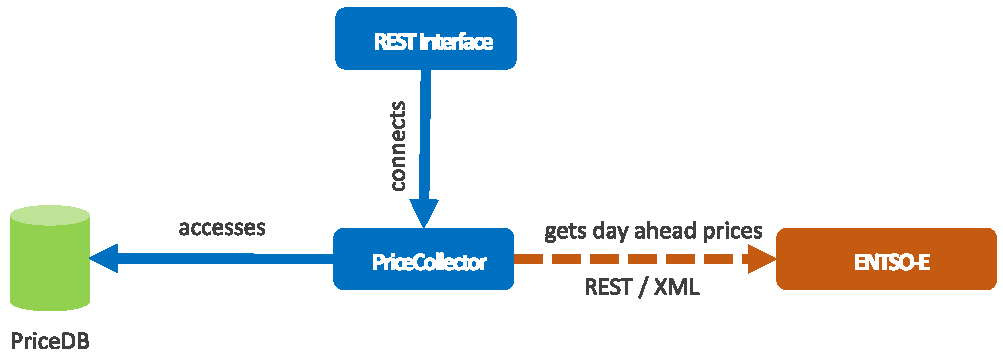
\includegraphics[width=1.00\textwidth]{../figures/priceCollector.pdf}
	\caption{Components: Price Collector}
	\label{fig:price}
\end{figure}
\noindent To fetch the data, we implemented an additional component which communicates with the API from ENTSO-E and manages database to store the data. \Cref{fig:price} contains an overview of the components used in your price collector. The price collector offers a REST Interface which uses JSON for the communication with the rest of our system. It communicates via an XML Format with the ENTSO-E REST Interface. It reads the data items from the API, filters them for the for us relevant data and saves them in an H2 Database. The necessary security token, the bidding zone and the port for the interface can be configured in a configuration file. The price collector has an auto-fetch feature which is also configurable and allows to request the ENTSO-E API in a user-defined pattern. For example, the day-ahead prices are published between 12 pm and 1 pm (one hour after gate closure) \cite{ENTSO3}. So it is possible to update the database each day at 1 pm. But also, more or less frequent patterns are possible. For example, each second hour. The price collector always tries to update its data with each request. If the ENTSO-E API is not available or it does not provide data for a specific period, the price collector uses older but still the most recent data from the database to fill the gaps. For example, if you request data for tomorrow at 4 pm and there is no data available from ENTSO-E the price collector will return the data from today at 4 pm. Such old data will be marked with a boolean flag in the response.    



\noindent We also updated your main architecture to reflect the new requirements. \Cref{fig:updatedA} showed the new architecture with the price collector. The database from the price collector is omitted in this figure. The Controller communicates via HTTP with the REST interface of the price collector. The price collector only offers one endpoint which is \glqq/prices\grqq{}. To make a request the start time and the end time of the required period have to be provided via query parameters. For all time-related information, the time zone UTC is used. 

\begin{figure}[htpb]
	\centering
	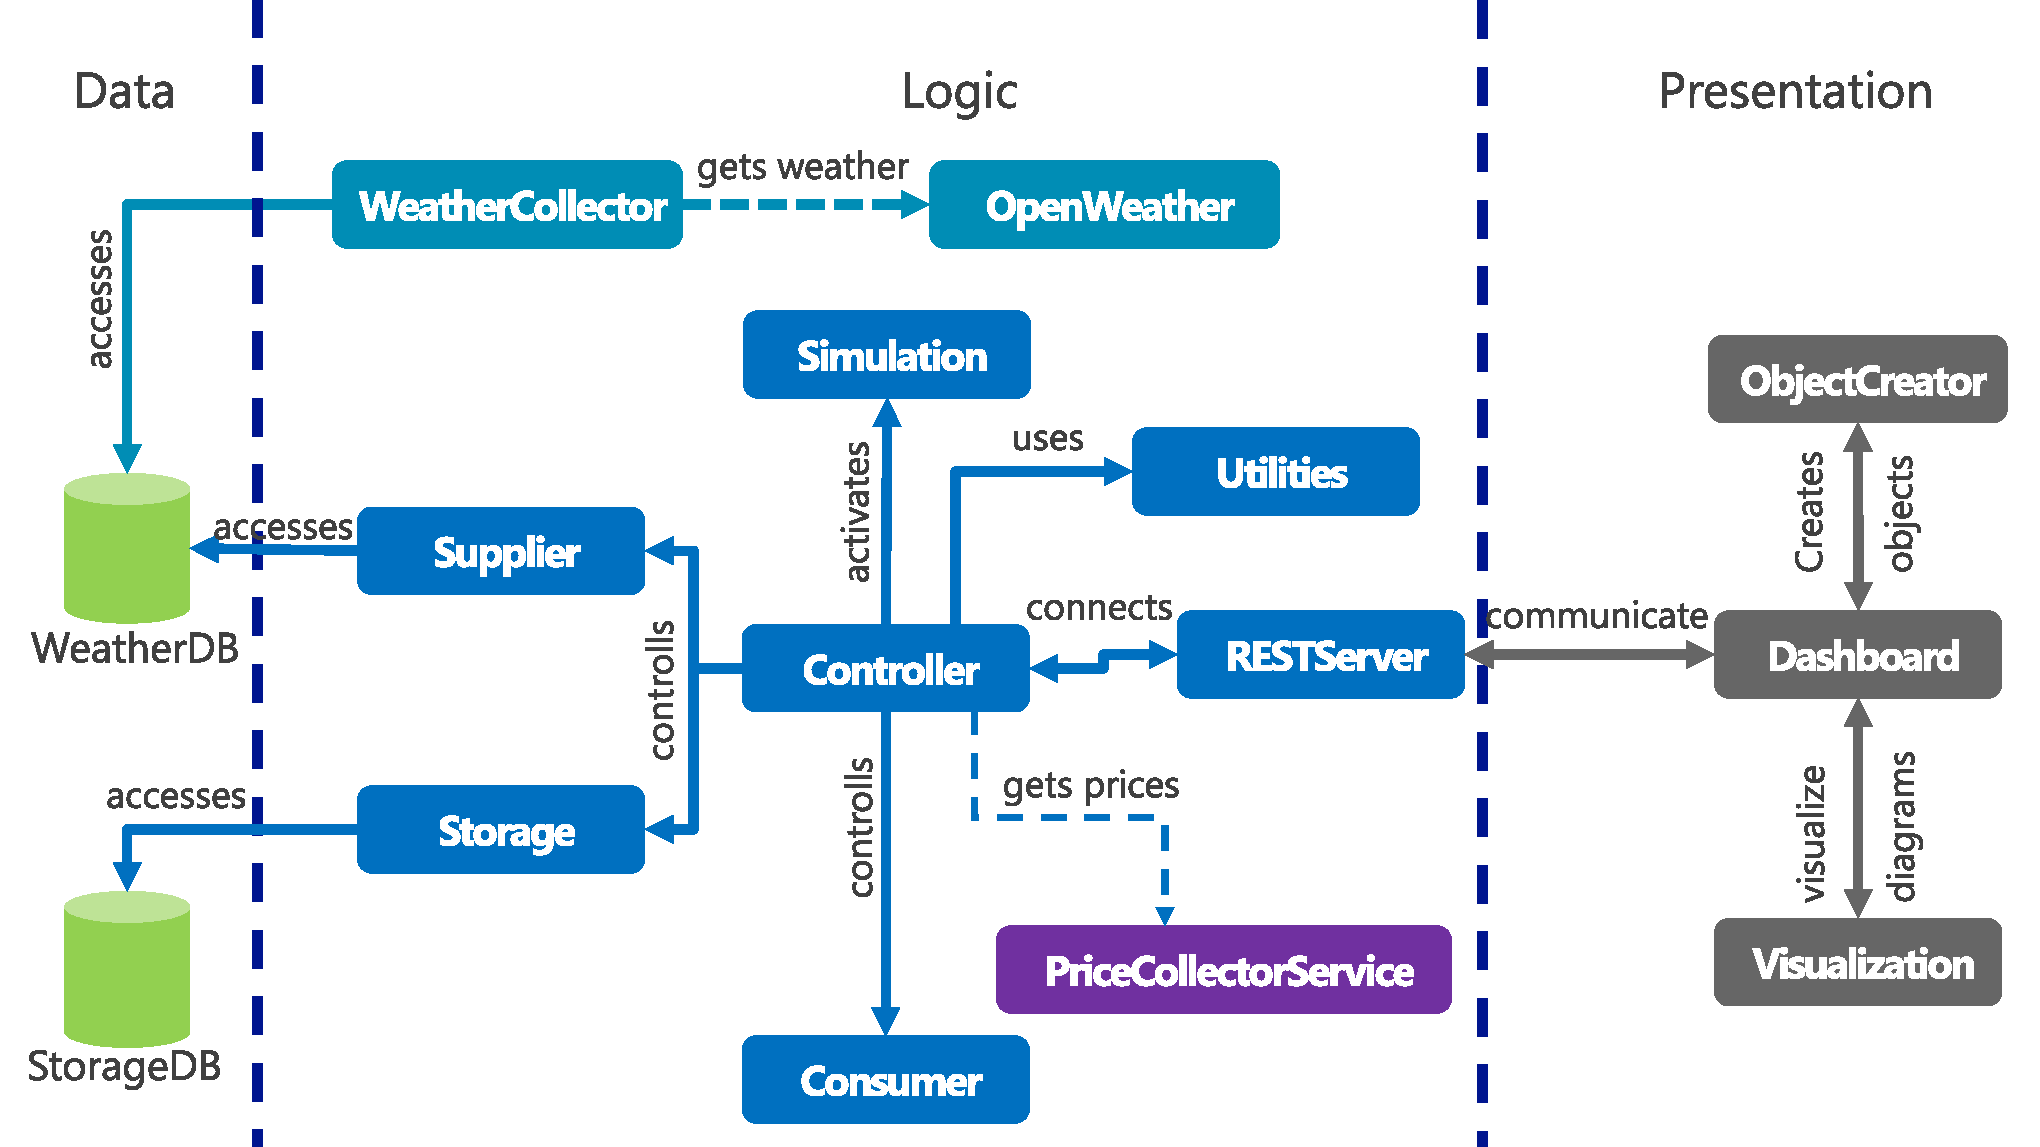
\includegraphics[width=1.00\textwidth]{../figures/Architecture2.pdf}
	\caption{Components: Price Collector}
	\label{fig:updatedA}
\end{figure}

\noindent The following figure contains an example snippet from an answer of our service. To use this answer our main system has to convert the information into the correct units. As always we provide a swagger documentation in the running competent.  

\begin{figure}[htpb]
	\centering
	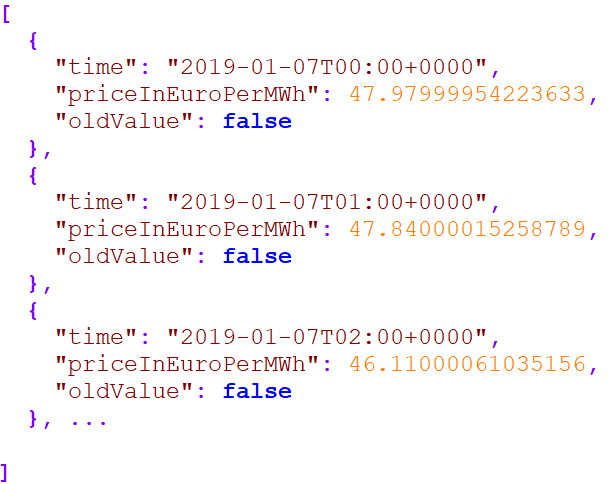
\includegraphics[width=0.5\textwidth]{../figures/response.png}
	\caption{Example response snippet}
	\label{fig:snipped}
\end{figure}
 
\noindent With this component, our system can simulate a microgrid and use real price data. We also added a test script to our repository to test the whole system. 
 \FloatBarrier

\section{Conclusions}
The power girds of the future will be different from the existing ones. More information will be used to make better decisions, more renewable energy sources will be integrated and more automation will happen. Also, microgrids will be a part of the energy concepts of the future. The simulation system presented in this report could help to gain a better understanding about different aspects of microgirds. The first section provided a motivation and introduction to microgirds. The next section contains basic information which are necessary to understand the problem, the functional requirements and an architecture description. The architecture is split in three layers. The webfrontend, the logic layer which contains the simulation and the database layer. It also features a reliable approach to integrate an external weather component. \Cref{sec:Implementation} contains a description of our implementation.\\

\noindent In the future more custom modules could be developed, to integrate even more suppliers and consumers.


\printbibliography
%\bibliographystyle{plain}
%\bibliography{bibliography}
All links were checked last on January 10, 2019.
% Ende des Dokuments
\end{document}
